\documentclass{article}
\usepackage{arxiv}
\usepackage[utf8]{inputenc}     % allow utf-8 input
\usepackage[T1]{fontenc}        % use 8-bit T1 fonts
\usepackage{hyperref}           % hyperlinks
\usepackage{url}                % simple URL typesetting
\usepackage{booktabs}           % professional-quality tables
\usepackage{amsfonts}           % blackboard math symbols
\usepackage{nicefrac}           % compact symbols for 1/2, etc.
\usepackage{microtype}          % microtypography
\usepackage{graphicx}
\usepackage{natbib}
\usepackage{doi}
\usepackage{xcolor}

\NewDocumentCommand{\code}{v}{\texttt{\textcolor{blue}{#1}}}

\title{ThreAIT: Using AI to Detect Prohibited Items in Airport X-ray Security Screening}

\date{December 4, 2023}

\author{
    \href{https://orcid.org/0000-0000-0000-0000}{Baris~Inandioglu} \\ 
        the Koç School \\
        Istanbul, Turkey \\
        \texttt{inandioglub@gmail.com}
    \And
    \href{https://orcid.org/0000-0003-2766-2816}{M. Ozgur~Sahin} \\
        CEA Irfu, Université Paris-Saclay \\
        Paris, France \\
        \texttt{ozgur.sahin@cern.ch}
}

\renewcommand{\shorttitle}{ThreAIT}

\hypersetup{
    pdftitle={ThreAIT: Using AI to Detect Prohibited Items in X-ray Security Screening},
    pdfsubject={cs.AI, cs.CR, cs.LG},
    pdfauthor={Baris~Inandioglu and M. Ozgur~Sahin},
    pdfkeywords={Anomaly detection, Convolutional Neural Networks, Transfer Learning, Image classification, Threat detection, Security screening, Machine learning, Deep learning, Computer vision, Pattern recognition, Classification algorithms, Feature extraction, Public safety, Neural networks, Unsupervised learning, Artificial intelligence},
}

\begin{document}

\maketitle

\begin{abstract}

In public safety, improving the security and efficiency of X-ray screening technology is imperative. This research report introduces ThreAIT, an advanced artificial intelligence (AI) system that autonomously detects prohibited items within airport X-ray scans. Given an X-ray scan image, ThreAIT binarily classifies the image, indicating the absence or presence of prohibited items within the inputted image. Central to ThreAIT's design is anomaly detection driven by convolutional neural networks (CNNs) and transfer learning. This paper introduces the working principles of ThreAIT and outlines the machine learning patterns and techniques used in its design.

\end{abstract}

\keywords{Anomaly detection \and Convolutional Neural Networks \and Transfer Learning \and Image classification \and Threat detection \and Security screening \and Machine learning \and Deep learning \and Computer vision \and Pattern recognition \and Classification algorithms \and Feature extraction \and Public safety \and Neural networks \and Unsupervised learning \and Artificial intelligence}

\newpage
\tableofcontents
\newpage

\section{Background: Machine learning and anomaly detection}

\subsection{X-ray Airport Security}
X-ray scans are widely used for security purposes. In these scans, objects appear with varying colors or shades depending on their density. Security personnel can analyze these images to detect items that may pose a security threat.

Traditional X-ray security screening involves human operators visually inspecting the images which might introduce human error. The introduction of artificial intelligence in the area, particularly Convolutional Neural Networks (CNNs), can automate the detection of prohibited items, mitigating human error. ThreAIT aims to utilize machine learning to detect X-ray scans of prohibited items.

\subsection{Machine Learning}
A machine learning algorithm aims to "learn" from raw data, as defined by Mitchell:

\begin{quote}
    “A computer program is said to learn from experience \(E\) with respect to some class of tasks \(T\) and performance measure \(P\), if its performance at tasks in \(T\), as measured by \(P\), improves with experience \(E\).” \cite{mitchell_machine_learning_book}
\end{quote}

\subsubsection{The Task}

The task is the end goal of the model. ThreAIT aims to use anomaly detection to perform binary classification on X-ray scans. Given a set of “normal” inputs, the computer is tasked to flag atypical data \cite{goodfellow_book}: X-ray scans with no prohibited items are "anomalous" when our model is trained using images of X-ray scans without prohibited items.

\subsubsection{The Experience}

In most cases, a training data set, a typically large set of example data (also called data points) is how an ML algorithm learns how to solve its task.

ML algorithms can be broadly categorized into three categories: Supervised learning, unsupervised learning, and reinforcement learning.

ThreAIT primarily employs unsupervised learning. This means that during the training process, the model learns to extract patterns from X-ray scans without requiring an explicitly labeled data set of anomalous data.

\subsubsection{The Performance Measure}
Even though the appropriate performance measure to use for any ML model is entirely dependent on its task, a simple but widely used measurement is the “accuracy” of the model. In ThreAIT, the accuracy of our model will be measured by how effectively it detects anomalies in the system.

\subsection{Neural Networks}

\subsubsection{Artificial Neural Networks}
Having explored the term “learning,” we can examine how machines make data-driven decisions by understanding neural networks: the building blocks of machine learning. According to Kelleher, a neural network is defined as:
“a computational model that is inspired by the structure of the human brain.” \cite{mit_book}

A biological neuron is a nerve cell found in the human central nervous system that responds to incoming stimuli by transmitting an electrical pulse. When chained through synapses, a large network of neurons can perform more complex tasks.

Artificial neurons take inputs from other neurons and produce an output signal, similar to the way the human brain functions with biological neurons. Similarly, by chaining artificial neurons, we can create an artificial neural network (ANN).

Both the human brain and ANNs are composed of interconnected units that collectively try to process information encoded as electrical signals.

\subsubsection{Convolutional Neural Networks}
A common type of artificial neural network, convolutional neural networks (CNNs) are especially useful for capturing intricate patterns within images through the use of convolutional layers. ThreAIT aims to classify a set of X-ray images, making CNNs the right architecture for the project. 

\subsection{Anomaly Detection}

ThreAIT utilizes anomaly detection to identify anomalous patterns within X-ray images autonomously.

The application of anomaly detection in ThreAIT involves binary classification of X-ray scans, where the model is trained to differentiate "normal" patterns from potential anomalies.

\section{ThreAIT}
\subsection{The Data Set}
The SIXray data set, curated by the Pattern Recognition and Intelligent System Development Laboratory at the University of Chinese Academy of Sciences, is utilized for training and evaluating ThreAIT. Comprising a repository of 1,059,231 X-ray images, this data set is appropriate for security inspection tasks.

The SIXray data set encompasses six common categories of prohibited items, including guns, knives, wrenches, pliers, scissors, and hammers.

\begin{figure}[h!]
    \centering
    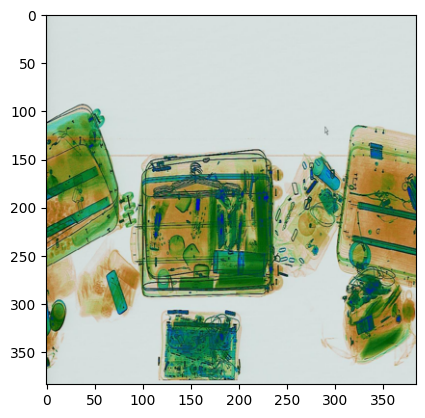
\includegraphics[width=0.75\linewidth]{img/example.png}
    \caption{Example image from the data set}
    \label{fig:example-image}
\end{figure}

\subsection{Data Extraction}

\subsubsection{Label Extraction}
The goal of label extraction is to locate and gather labels connected to signal events—anomalous patterns in the X-ray pictures. Labels are extracted to create an exhaustive list of signal events from paths that are supplied and contain related XML files. These labels are annotations that the model uses during training. They help the machine learning algorithm identify and categorize patterns in the X-ray scans that indicate the presence of prohibited items. The accurate extraction of these labels improves the model's capacity to distinguish abnormal from normal data, thereby improving the model accuracy.

\subsection{Image Processing}
\subsubsection{Contour Detection}
 
ThreAIT employs contour detection to reduce noise and improve model output. Identifying and delineating the boundaries of objects within X-ray scans enhances the model's ability to discern shapes and structures.

\begin{figure}[h!]
    \centering
    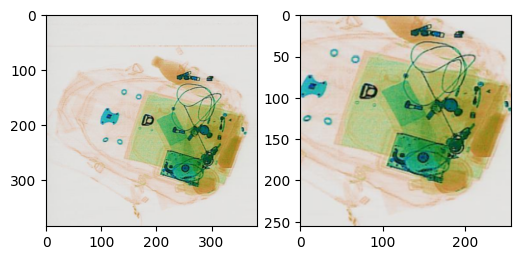
\includegraphics[width=1\linewidth]{img/contour.png}
    \caption{Image before and after contour detection}
    \label{fig:contour-before-after}
\end{figure}

\subsection{The Model Architecture}
Comprising of two main components, the encoder and decoder, the model leverages transfer learning principles for enhanced feature extraction.

The encoder is constructed based on the pre-trained EfficientNetV2M convolutional neural network. Transfer learning is a pivotal aspect of the encoder's functionality, allowing ThreAIT to repurpose knowledge gained from general-purpose image recognition to the specific task of anomaly detection. This process helps extract relevant features from X-ray scan images. After the encoding process, the encoded data is passed to the decoder model which aims to reconstruct the encoded data. 

\subsection{The Encoder}
The encoder module plays a pivotal role in ThreAIT's architecture, employing transfer learning to leverage pre-trained models for efficient feature extraction. Transfer learning involves utilizing knowledge gained from training on one task (e.g., image classification on a diverse data set) and applying it to a different but related task (anomaly detection in X-ray scans).

\subsubsection{The Encoder Summary}
\begin{verbatim}
__________________________________________________________________________________________________
 Layer (type)                Output Shape                 Param #   Connected to                  
==================================================================================================
 input_7 (InputLayer)        [(None, 256, 256, 3)]        0         []                            
 efficientnetv2-m (Function  (None, 8, 8, 1280)           5315038   ['input_7[0][0]']             
 al)                                                      8                                       
 conv2d_4 (Conv2D)           (None, 8, 8, 256)            2949376   ['efficientnetv2-m[0][0]']    
 conv2d_5 (Conv2D)           (None, 8, 8, 128)            295040    ['conv2d_4[0][0]']            
 flatten_2 (Flatten)         (None, 8192)                 0         ['conv2d_5[0][0]']            
 dropout_2 (Dropout)         (None, 8192)                 0         ['flatten_2[0][0]']           
 dense_6 (Dense)             (None, 2048)                 1677926   ['dropout_2[0][0]']           
                                                          4                                       
 dense_7 (Dense)             (None, 2048)                 1677926   ['dropout_2[0][0]']           
                                                          4                                       
 tf.compat.v1.shape_4 (TFOp  (2,)                         0         ['dense_6[0][0]']             
 Lambda)                                                                                          
 tf.compat.v1.shape_5 (TFOp  (2,)                         0         ['dense_6[0][0]']             
 Lambda)                                                                                          
 tf.math.multiply_4 (TFOpLa  (None, 2048)                 0         ['dense_7[0][0]']             
 mbda)                                                                                            
 tf.__operators__.getitem_4  ()                           0         ['tf.compat.v1.shape_4[0][0]']
  (SlicingOpLambda)                                                                               
 tf.__operators__.getitem_5  ()                           0         ['tf.compat.v1.shape_5[0][0]']
  (SlicingOpLambda)                                                                               
 tf.math.exp_2 (TFOpLambda)  (None, 2048)                 0         ['tf.math.multiply_4[0][0]']  
 tf.random.normal_2 (TFOpLa  (None, 2048)                 0         ['tf.__operators__.getitem_4[0
 mbda)                                                              ][0]',                        
                                                                     'tf.__operators__.getitem_5[0
                                                                    ][0]']                        
 tf.math.multiply_5 (TFOpLa  (None, 2048)                 0         ['tf.math.exp_2[0][0]',       
 mbda)                                                               'tf.random.normal_2[0][0]']  
 tf.__operators__.add_2 (TF  (None, 2048)                 0         ['dense_6[0][0]',             
 OpLambda)                                                           'tf.math.multiply_5[0][0]']  
==================================================================================================
Total params: 89953332 (343.14 MB)
Trainable params: 36802944 (140.39 MB)
Non-trainable params: 53150388 (202.75 MB)
__________________________________________________________________________________________________
\end{verbatim}

\subsubsection{Transfer Learning}
Transfer learning is a machine learning approach where a pre-trained model is repurposed to improve performance on a different but related task.

ThreAIT employs transfer learning by using the EfficientNetV2M pre-trained model, initially designed for general-purpose image recognition, in its model. This approach allows the model to capture complex patterns and hierarchical features inherent in image data sets, contributing to its ability to discern anomalies in X-ray scans effectively.

\subsection{The Decoder}
The decoder component in ThreAIT reconstructs the encoded representations from the encoder into meaningful output. This process involves decoding the learned features back into the spatial structure of the original X-ray scans. The decoder architecture is tailored to reverse the compression performed by the encoder. Through this reconstruction, ThreAIT aims to represent the input images, enabling anomaly detection by comparing the reconstructed scans with the originals.

\subsubsection{The Decoder Summary}
\begin{verbatim}
_________________________________________________________________
 Layer (type)                Output Shape              Param #   
=================================================================
 input_9 (InputLayer)        [(None, 2048)]            0         
 dense_8 (Dense)             (None, 131072)            268566528 
 reshape_2 (Reshape)         (None, 32, 32, 128)       0         
 conv2d_transpose_8 (Conv2D  (None, 64, 64, 64)        73792     
 Transpose)                                                      
 conv2d_transpose_9 (Conv2D  (None, 128, 128, 32)      18464     
 Transpose)                                                      
 conv2d_transpose_10 (Conv2  (None, 256, 256, 16)      4624      
 DTranspose)                                                     
 conv2d_transpose_11 (Conv2  (None, 256, 256, 3)       435       
 DTranspose)                                                     
 rescaling_5 (Rescaling)     (None, 256, 256, 3)       0         
=================================================================
Total params: 268663843 (1.00 GB)
Trainable params: 268663843 (1.00 GB)
Non-trainable params: 0 (0.00 Byte)
_________________________________________________________________
\end{verbatim}

\newpage
\bibliographystyle{ieeetr}
\bibliography{references}

\end{document}